\documentclass[a4paper,10pt,lithuanian]{article}

\usepackage{lnfkstyle}

\begin{document}

\titlelt{Pavadinimas lietuvių kalba}

\titleen{Pavadinimas anglų kalba}


\author{\uline{Vardis Pavardis}$^{1}$, Vardžius Pavardėnas$^{1,2}$}

\keywords{potencialas, kinetika, elektrinio lauko stipris}

\maketitle

\address{$^{1}$Vilniaus universitetas, Fizikos fakultetas, Saulėtekio al. 9, 10222 Vilnius}

\address{$^{2}$Fizinių ir technologijos mokslų centras, Savanorių pr. 231, 02300 Vilnius}

\rightaddress{vardas.pavardis@pastas.lt}

\begin{multicols*}{2}
Lietuvos nacionalinės fizikos konferencijos dalyviai pateikia \textbf{vieno}, nemažiau 80\% užpildyto, \textbf{puslapio} tezes. Priimamos \textbf{tik PDF formato} tezės. Visi šriftai turi būti romaninio tipo (jei naudojate MS Word arba OpenOffice -- Times New Roman, \LaTeX -- Computer Modern Roman). Tezėse turi būti pateiktas pranešimo pavadinimas lietuvių ir anglų kalba (12 pt. dydžio, pastorintas), autorių vardai ir pavardės, jų institucijų adresai, elektroninio pašto adresas susirašinėjimui (10 pt. dydžio, įprasto storio). Pranešėjo vardas ir pavardė turi būti \uline{pabraukti}. Teksto pabaigoje turi būti pateikti reikšminiai žodžiai, o po jų gali būti literatūros sąrašas iš ne daugiau 5 šaltinių (8 pt. dydžio).

Tezės turi būti pateiktos lietuvių kalba. Kai vienas ar keli bendraautoriai yra užsieniečiai, tezes galima pateikti anglų kalba.

\textbf{A4 formato lape} teksto maketavimas turi būti \textbf{dviejų stulpelių}. Kiekvieno stulpelio plotis turi būti 8 cm, tarpas tarp stulpelių turi būti lygus 1 cm. Kairės ir dešinės pusės paraštės turi būti 2 cm, o viršaus ir apačios -- 2,5 cm. \textbf{Nenumeruokite puslapio}.

Tezių teksto šriftas turi būti 10 pt. dydžio su vienu eilėtarpiu (\textit{single spacing}).

Matematinės išraiškos turi būti numeruotos eilutės pabaigoje. Simbolių didumas matematinėse išraiškose turi būti toks pat kaip ir tekste. Primename, kad kintamieji dydžiai bei funkcijos simboliai rašomi \textit{pasviru}, o matematinės funkcijos ($\sin$, $\exp$, etc.), konstantos ($\mathrm{e}$, $\mathrm{i}$, etc.), diferencialo ženklas ($\mathrm{d}$) ir žodžių sutrumpinimai -- įprastu (statmenu) šriftu:
\begin{equation}
I_\mathrm{s}\approx\left( \frac{I_0k_\mathrm{B}T}{\pi h} \right) \int \frac{f_0\gamma}{(\omega^2-\omega_0^2)^2+\gamma^2\omega^2} \mathrm{d}\omega
\end{equation}

Paveikslų matmenys turėtų būti parinkti taip, kad neviršytų vieno stulpelio pločio. Atkreipkite dėmesį į simbolių indeksų didumą formulėse ir paveiksluose -- jie turėtų būti gerai įskaitomi.

Lenteles ir paveikslus numeruokite pagal pasirodymo tekste eiliškumą.

\vspace{10pt} \noindent 1 lentelė. Dydžių $\omega$ ir $\gamma$ įprastinės vertės, esant skirtingoms temperatūroms.
\begin{center}
\begin{tabular}{ccc}
\hline
$T$ (K) & $\omega$ (GHz) & $\gamma$ (GHz) \\
\hline
420 & 15,3 & 7,8 \\
400 & 16,0 & 6,9 \\
370 & 18,4 & 5,0 \\
320 & 20,2 & 2,1 \\
\hline
\end{tabular}
\end{center}

Cituojamos literatūros sąrašas pateikiamas teksto pabaigoje po reikšminių žodžių\cite{key-1}. Sąrašas turi būti numeruojamas pagal pasirodymo tekste eiliškumą\cite{key-2}.

Elektronines tezių versijas siųskite naudodami automatinę tezių siuntimo sistemą konferencijos puslapyje 
\uline{http://lnfk.ftmc.lt}

Konferencijos tezės bus priimamos \textbf{iki 2015 m. balandžio 24 dienos}.

Visos pateiktos tezės bus peržiūrimos. Netvarkingai apipavidalintos tezės bus grąžinamos autoriams pataisyti.
Tezių medžiaga bus talpinama internete.

\begin{center}
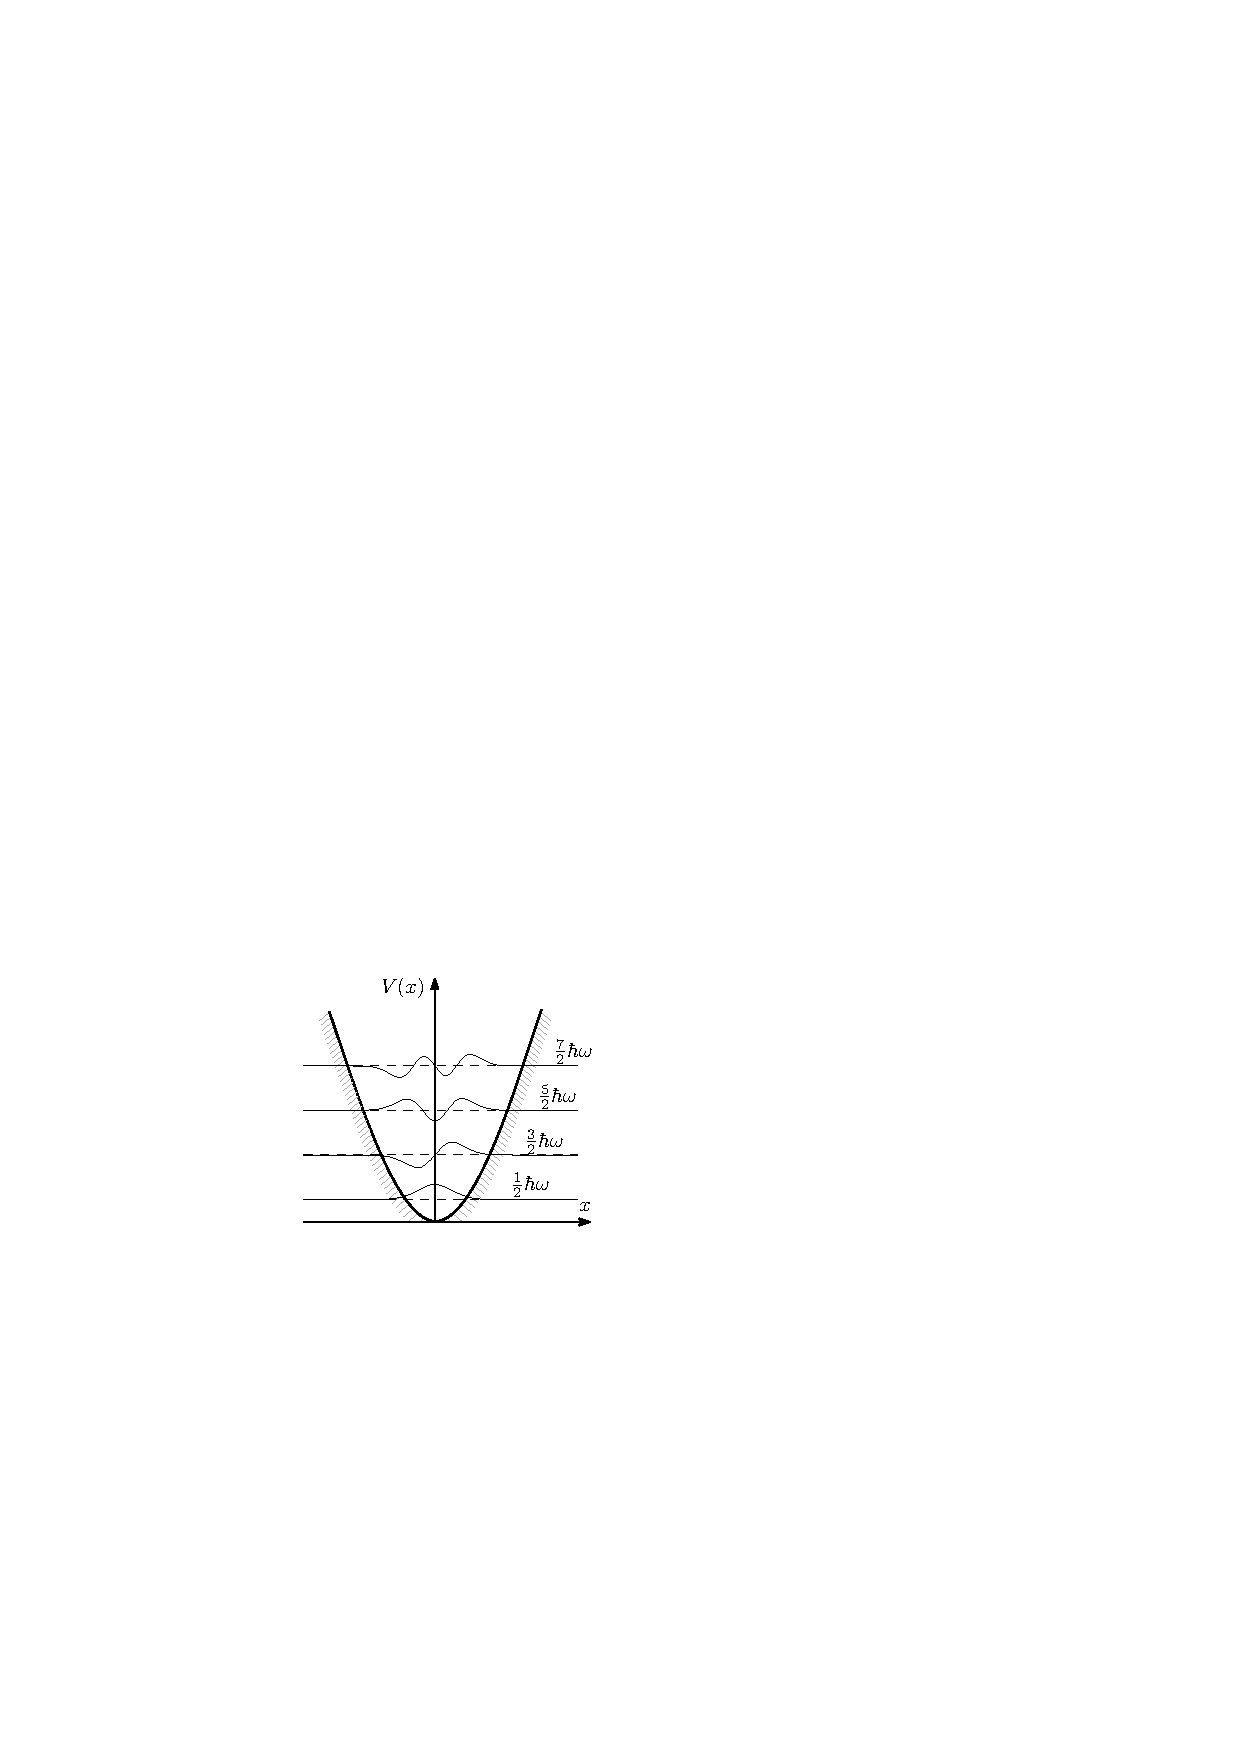
\includegraphics{paveikslas.pdf}

1 pav. Kvantinio harmoninis osciliatoriaus potencinė energija ir kelios banginės funkcijos.\vspace{10pt}
\end{center}

\begin{thebibliography}{References}

\bibitem{key-1}S. G. Lushnikov, J.-H. Ko, and S. Kojima, Appl. Phys. Lett. \textbf{84}, 4798 (2004).

\bibitem{key-2}P. M. Boersenberger, D. S. Weiss, \textit{Organic Photoreceptors for Imaging Systems} (New York, Besel, Hong Kong, 1993).
\end{thebibliography}

\end{multicols*}
\end{document}
